\chapter{Development}

Initially, if we have a non empty graph, we can act as if the graph is static and let HyperBall perform a complete calculation on it. This should be a very fast operation as HyperBall is highly optimized for static graphs. After HyperBall has completed, we can use the calculated counters as initial counters for our dynamic algorithm. For every insertion and deletion in the dynamic graph, these initial counters are manipulated. If an edge is added, nodes might reach more nodes than before and their counters should be raised. Similarly for deletions, if an edge is deleted, nodes might reach fewer nodes and their counters should be decreased. \todo{More intro or enough?}


\section{Dynamic graphs}

The first thing we need for a dynamic graph is the ability to insert new nodes and edges (called entries in this section) to an existing graph. The graph files used by HyperBall are tightly compressed in a byte stream, which makes it an expensive operation to modify the graph at an arbitrary point. This makes it infeasible to insert every additional entry directly into the graph file. Instead, new entries can be stored in some other data structure.

The additional entries could either be stored in a high-level data structure or some sort of byte stream. Keeping them in a high-level data structure will consume a significant amount of storage already at a low number of extra entries. A high-level data structure takes up more memory as each number is always the same size no matter what the value is. Additionally, if each node has a structure containing the neighbors, a significant amount of space will be taken by the pointers to those structures. The compression of the graph is also lost when using a high-level structure.

If a byte stream is used, we get to the same problem as the original. Even though this byte stream will be smaller, there will be a point where it is unreasonable to resize the stream and reposition the existing entries at each new entry. Regardless of which method we use we have to merge the extra entries and the original graph to a new graph at some point. 

\subsection{Merging two graphs with webgraph}

The webgraph framework has a way to create a new graph $G'$ by taking the union of two sub graphs $G_1$ and $G_2$. The graph $G'$ works by simultaneously reading from the streams of $G_1$ and $G_2$ to produce the nodes and their neighbors. The sub graphs can be unions as well which means that one can join an arbitrary number of graphs using this method. However, having lots of recursive unions create a large overhead in time \todo{SOME TESTS SHOULD BE DONE ON THIS}when fetching nodes and edges. \cite{webgraph} 

The framework also supports writing a union-graph to disk as a new graph. Loading this new written graph removes the overhead of several recursive unions. As the graph express some arcs by references to previous arcs the creation is slow and doesn't leverage any of the calculations already made by the existing graphs. Ignoring the references will make the graphs bigger but it increases the running time of the merge. 

\subsection{Merging two graph files}
A method to merge the raw format of two BVGraphs without the references has been developed. The speed improves by \todo{Benchmark}several tens by ignoring the references and the space taken by the graphs are around twice as much. Our merge method is more appropriate than the existing one as for the algorithm to be dynamic we have to be able to modify the graphs quickly. It has two phases for each node. The first phase reads the intervals of both graphs and merges them as much as possible. As the intervals in the files are sorted in ascending order by the start of the interval, this can be done in $O(n)$ time (see Appendix B). In the next step the algorithm takes the smallest residual node from one of the graphs and writes it to the output graph. As the residuals are already sorted in ascending order in the graphs we only need to look at the first residual in the lists. If they are the same, it is written once and both file pointers are moved forward so that no duplicates are written. If the residual to be written is already included in one of the intervals, it is ignored. Using the developed method allows us to merge very large graphs at a short amount of time.

\subsection{How we solved it}
Not completed yet

\section{HyperLogLog resize}
After new nodes have been added to the graph we need to allocate new counters for them. The initial counters we get from HyperBall are represented as an array of longs. We intend to keep this representation, as it has a very low amount of wasted memory usage. It also minimized the number of objects created on the heap. But as new counters are needed, we must resize the array. For this, we use a geometric expansion as it gives $O(1)$ amortized time per insertion \cite{dynamicarrays}. In the geometric expansion we increase the array capacity by a factor. This is how the standard implementation of ArrayList in Java is dynamically increased. A larger factor implies an on average small number of copies per inserted elements but a high amount of unused space. The amortized number of copies per inserted element for a factor $r$ is roughly $\frac{1}{(r-1)}$ and the average unused space is $\log(r)*\frac{r}{(r-1)} - 1$. \cite{dynamicarrays}

Under the assumption that the graph expands slowly relative to its size \todo{Where is this assumption? write in problem description what assumptions we have, eg expands, delete/insert ration}, resizing events will be sparse and a large factor would mainly imply a large amount of unused memory. Therefore, we made the choice to let the array increase by a small factor. With the factor $r = 1.1$ we get an average of $4.8$\% of unused space and $10$ copies per insertion. 

\section{Updating counters}

After an edge have been added to the graph, the next step is to update the counters of all nodes affected by the insertion.  Let $e = (u,v)$ be an edge added to the graph. All the nodes reachable from $v$ now have to be propagated to the nodes that now can reach $v$ via $u$. This is performed in two phases, the collecting-bfs and the propagating-bfs. 

The collecting-bfs is responsible for retrieving which nodes $v$ can reach. The collecting-bfs performs a bfs in the graph from $v$. For every level $i$ in the bfs, all nodes in the current frontier in the bfs are added into a HyperLogLog counter, which represents all nodes that $v$ reached in $i$ steps. The collecting-bfs completes at level $h-1$ and returns a $h$ long list of counters. The $h$'th step is not needed as only $v$ itself can reach this level. 

The propagation-bfs is responsible for updating the counters of all nodes that now reach $v$, as they might have changed by the insertion. To find all nodes that can reach $v$, a bfs is performed from $u$ in the transpose of the graph. For every level $i$ in the bfs, the frontier of nodes in the bfs can reach all nodes that the collecting-bfs reached in $h-1-i$ steps. To update the counters of the nodes at level $i$, the current counters of the nodes are merged with the $h-1-i$ counter retrieved in the collecting-bfs. The propagation-bfs stops after $h-1$ steps after which all affected node counters have been updated.  

\todo{Do we want some simple proof here of correctness?}

\subsection{Optimized Breadth-first search}

A problem with the two phase algorithm described above is that it only supports single insertions at a time. Instead of adding each edge separately, they can be bulked into a set of edges to add. By bulking the edges we can do several BFS's at the same time. The algorithm MS-BFS \cite{msbfs} does several BFS's at the same time very effectively and will be used in the algorithm. \todo{Show benchmark between std bfs and ms-bfs}

As the BFS can be pruned when we have traversed $h-1$ steps we need a way to stop the individual BFS's at that point. To solve this we have implemented a method to pass the MS-BFS a visitor function (not related to the common Visitor design pattern). The visitor will be called every time a bunch of BFS's have reached a node. The group of BFS's that reached the node is represented as a list of bits and is passed to the visitor. If the visitor wants to stop the propagation of a BFS from this node it can clear the corresponding bit. No modifications to the algorithm needs to be done as MS-BFS already use a list of bits to propagate the BFS's.

We want to send data along with the BFS's. This leads us to introduce a new concept called travelers. The purpose of the traveler is to bring initial data from the BFS's and merge the data if several BFS's reach a node at the same time. This may prevent calculations that would otherwise need to be done in all or many of the visitors by removing the need to loop through which source nodes that reached the node. Travelers have to be able to merge to not increase the space complexity of the algorithm. The traveler is then passed to the visitors so they can use the data provided by the travelers. 

\section{Node history}

MS-BFS speeds up the algorithm significantly, but further optimizations can be done to the individual BFS's. To update a counter, the algorithm has to do two BFS's for every edge added. A large portion of the time spent by the algorithm will be doing these BFS's. Therefore, the ability to prune BFS's early would imply a large time improvement of the run time. Currently, a BFS must search $h$ steps to gather all data needed to calculate its neighborhood function. This is because every node only keeps track of its registers resulted by a search in $h$ steps. But if all nodes keep track of its registers in $h-1$ steps, then the collecting-BFS would only need to traverse $h-1$ steps as in the $h-1$'th step it could use the $h-1$ history of all nodes to calculate the $h$'th step. For every extra history level we add, the collecting-BFS can stop one step earlier. So by saving every history level of all nodes, the collecting-BFS only needs to visit the immediate neighbors of an updated node $v$ to be able to calculate the counter of $v$. 

During the HyperBall phase of the algorithm, the intermediate counters in HyperBall can be used to calculate all history levels of all nodes. HyperBall works in iterations, synchronizing all nodes between every step taken. During the $i$'th synchronization, the counters will represent the $i$'th level of all nodes history and instead of only saving level $h$, we save all levels. We will refer to level $h$ as the top counter, level $0 - (h-1)$ as history counters and all levels together as counter collection.  

Every node now has a list of its history which has to be updated with every edge update. For an edge $e = (u,v)$ inserted, the collecting-BFS has to gather the node history from all neighbors of $v$ and merge them into one. The merged history together with the $v$ itself added to them becomes $v$'s own history and counter. Then the propagation-BFS has to propagate this history in the transpose of the graph. These extra operations can be performed during the current BFS's and should not affect the algorithms running time very much.

With node history we get $O(hn \log \log n)$ space complexity as the top counter uses $O(n \log \log n)$ and the history counters use $O((h-1)n \log \log n)$. To insert an edge $e = (u,v)$, the two previous BFS's used $O(m)$ operations per BFS but with node history the collection-BFS use $O(\Delta_v)$ operations, where $\Delta_v$ is the outdegree of node $v$. The time complexity of the node history version is then $O(m + \Delta_v)$. In practice, this means a large improvement as it often holds that $\Delta_v < m$.

Node history gives us a faster algorithm but also an extra space consumption that, for large graphs, can be quite extensive. To create a  algorithm that balances the gained speed versus the extra memory usage we could save the history of only a subset of nodes. These nodes should be picked so that as few nodes as possible need to save their history while keeping the BFS distance as short as possible. The algorithm to determine these nodes have to be very fast to avoid affecting the running time of the algorithm too much. It would also have to be dynamic to be able to continuously determine which nodes that should be included in the set.

\subsection{Vertex cover}
One way to determine which nodes that should keep their history is to use the nodes that are in a minimum vertex cover $VC$. Only saving the node history on nodes that are part of the $VC$ can significantly improve space usage, yet the BFS can still be bounded. The trick here is that for all nodes $u$, we know that $u \in VC \vee \forall e = (u,v) : v \in VC$. Then, when the collecting-BFS searches from a node $v$ it will take at most two steps until we get a frontier of only nodes in the vertex cover. From this frontier, the collecting-BFS can calculate $v$'s history and counter by merging the frontier histories. The collection-BFS is now bounded by two steps, resulting in $O(\Delta_v + \sum_{u \in \delta^+_v}{\Delta_u}) $ operations. The top counter uses the same space but the history counters now use $O((h-1)|VC| \log \log n)$, so the total space complexity for the counter collection is $O(((h-1)|VC| + 1 )\log \log n)$.


\subsubsection{Dynamic minimum vertex cover}
We now have the requirement that we at all times need to keep track of which nodes are in the vertex cover. This requires a fully dynamic minimum vertex cover algorithm. However, as minimum vertex cover is NP-complete, we need to resort to approximation algorithms. The choice of fully dynamic approximate minimum vertex cover algorithm depends on the ratio between the number of insertions and deletions. A simple greedy algorithm can maintain a $2$-approximation in $O(1)$ time per insertion and $O(n)$ time per deletion \cite{2appdynvc}, while an algorithm that partition the nodes can maintain the same approximation in $O(\log(n))$ amortized time per insertion and deletion \cite{2appdynvclogn}. In our case, \todo{state this in problem description or something} deletions will be very sparse in the data stream, which is why we chose the greedy algorithm. The greedy algorithm also have the property that if a deleted edge was not part of the maximal matching previously, it deletes the edge in $O(1)$ operations. For dense graphs, only a small amount of the edges will be in the maximal matching, which makes it in many cases perform very quickly in deletions as well. 

 
\subsubsection{Directed graphs}
As the standard minimum vertex cover problem is defined for undirected graphs we have to slightly modify the problem. Our problem description is as follows; given a directed graph $G = (V,E)$, we wish to select a minimum cardinality subset $V' \subseteq V$ such that $\forall e = (u,v) \in E, u \in V' \vee v \in V'$. The problem is still NP-complete as undirected graphs are a special case of directed graphs. 

By the same reasoning as in the undirected case, a maximal matching is a $2$-approximation of the generalized problem. However, the greedy algorithm needs to be modified to support directed edges. The only case affected is when an edge in the maximal matching is deleted. Previously, the algorithm scanned the endpoints of the deleted edge for uncovered edges. With directed edges we must verify both incoming and outgoing edges. This can be solved by saving both directions into each node, as in the undirected case. However, as we are dealing with large graphs we wish to minimize the amount of memory used per node. Also, as we expect deletions to be rare, saving both types would in most cases be unnecessary. Instead, we resort to scanning all the edges to find affected edges. This requires no extra information added, but implies a larger time complexity for deletions. Instead of $O(n)$ we now get $O(m)$ per deletion. Fortunately, we can reduce the amortized number of edge scans required per deletion by performing deletions in bulk. A single edge scan is sufficient for detecting all the affected edges of any sized bulk of deletions. So by utilizing bulk deletions we can minimize the number of edge scans.

\subsubsection{Benchmark}
See figure \ref{fig:firstIterationDvc} \todo{Write something here eheh}

\begin{figure}[h]
\centering
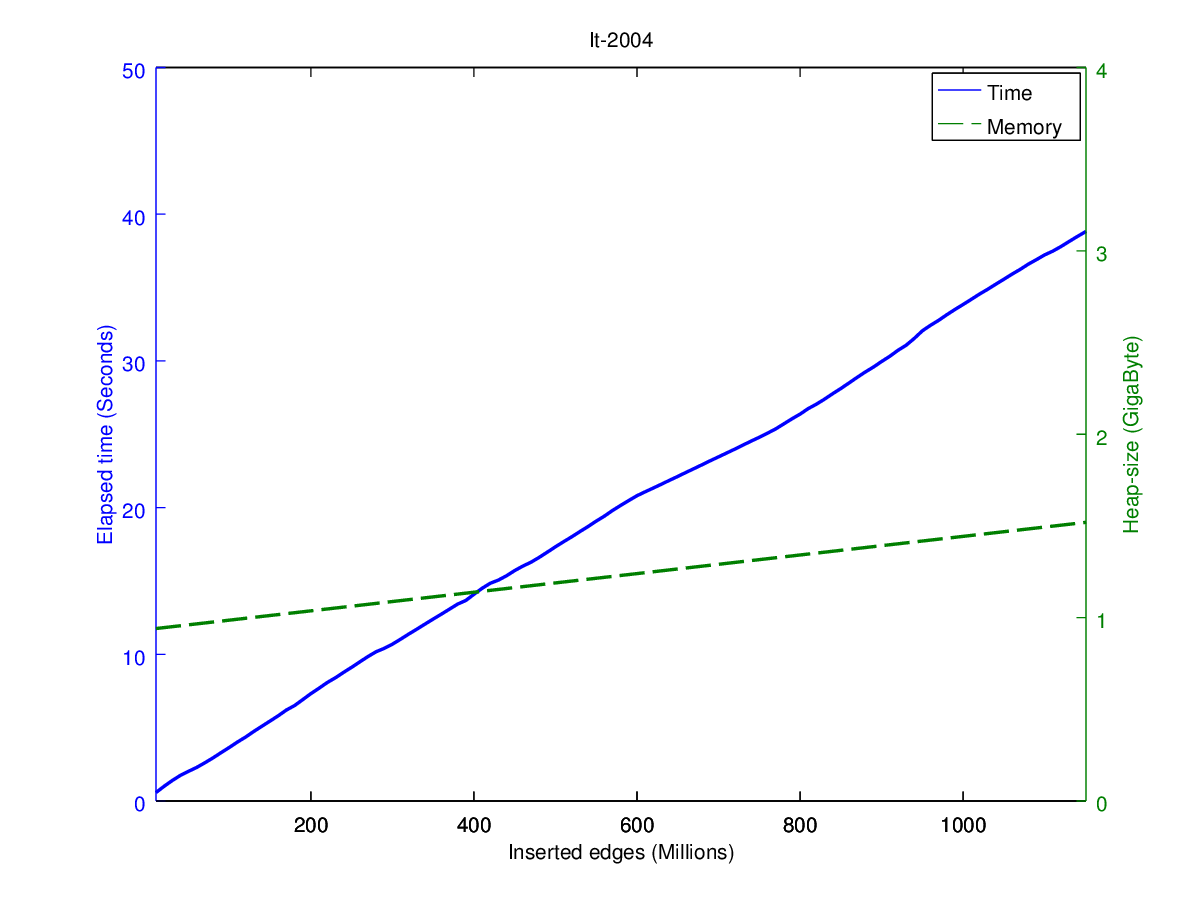
\includegraphics[width=15cm]{firstIterationDvc}    
\captionsetup{justification=centering}
\caption {Benchmark of insertions in 2-approximative dynamic vertex cover}
\label{fig:firstIterationDvc}
\end{figure}


\section{Algorithm}

\todo{This section mention lots of already mentioned things. perhaps we should check this over}

As the algorithm should be able to be initiated on an existing graph we use HyperANF to calculate the initial counter collection. HyperANF is already implemented in an iteration based manner. For each iteration run, the neighborhood function for all nodes reach one step further. The counters for the nodes in the vertex cover are extracted for each iteration, except the last iteration where we keep all nodes counters. \todo{perhaps this will be similar to Node History when we describe it more}

\subsection{Edge Insertions}

Edge insertion is divided into four steps. The first step is checking if the edge contains nodes not present in the current graph. New nodes are added to the graph and the top counter is, if necessary, resized to fit new counters of the new nodes. The second step is to check if any new node needs to be added into the vertex cover. For all new nodes in the vertex cover, memory is allocated in the history counters. The third step is calculating the history of the nodes added to the vertex cover. Lastly, the new history is propagated with a BFS in the transpose graph to update the counters of nodes that reach new nodes. After these four steps all nodes will have their top counters updated and all nodes in the vertex cover will have their history counters in order. 

\subsubsection{Calculating node history}

Calculating the node history of an added node $v$ is done based on the history from the vertex cover nodes around $v$. We know that there will be a vertex cover node on all paths at most 2 steps away. We perform a BFS from $v$. If it encounters a node $u$ not in the vertex cover, $u$ is simply added to the counter of $v$. This can only happen at one step away from $v$, so $u$ is added to all counters in $v$'s history except the top one. If a node $u$ that is in the vertex cover is encountered we can take the history-counters of $u$. Let the distance from $u$ to $v$ be $x$. We take the counters on level $0$ to $h-x$ from $u$ and union them with the top history counters of $v$. \todo{This sentence can probably be better structured}  The algorithm in pseudo-code:

\todo{Should be h instead of i?, second row}
\begin{figure}[h]
    \begin{lstlisting}[mathescape]
v = The node to calculate the history for;
H(v,i) = the neighborhood function for v reaching i steps;
In BFS; current node: u, at depth: d > 0{
    if(isInVertexCover(u)){
        for all i: d $\leq$ i $\leq$ h {
            H(v,i).union(H(u,i-d));
        }
        //prune this BFS branch
    }else{
        H(v,h-1).add(u);
    }
}
    \end{lstlisting}
    \caption{Edge insertion algorithm}
    \label{fig:edge_insertion_algorithm}
\end{figure}

The algorithm only works for one node at a time. However, by leveraging the mentioned MS-BFS algorithm \cite{msbfs}, we can perform the calculation for several nodes at the same time. When using MS-BFS we get a list the source nodes that reach the node with the given depth. The new algorithm becomes:

\begin{figure}[h]
    \begin{lstlisting}[mathescape]
H(v,i) = the neighborhood function for v reaching i steps;
In BFS; sources: V, current node: u, at depth: d > 0{
    foreach v $\in$ V{
        if(isInVertexCover(u)){
            for all i: d $\leq$ i $\leq$ h {
                H(v,i).union(H(u,i-d));
            }
            //prune this BFS branch
        }else{
            H(v,h-1).add(u);
        }
    }
}
    \end{lstlisting}
    \caption{Multiple edge insertion algorithm}
    \label{fig:multiple_edge_insertion_algorithm}
\end{figure}

Unfortunately this algorithm is not thread-safe. For example if two threads are running the union method for the same node at the same time it is very likely that one of the calculations are lost. Large portions of the BFS will still be done in parallel. There are several ways to synchronize the calculation which may allow large parts of the visitor to be done in parallel. Experiments with different synchronizations will be made in the Benchmarking section. Another bad property is that the BFS can arrive at one of the new nodes which may not have finished its history calculation. However, the fourth step in the algorithm, the propagation step, will solve this issue. 

\subsubsection{History propagation}

When a new edge $e = (u,v)$ is added to the graph, many nodes that has a path to $u$ will contain outdated information. The algorithm works by propagating the history of $v$ through the transpose of the graph. If $v$ is not in the Vertex Cover we need to calculate its history from the neighbor nodes. We present the algorithm as pseudo code:

\todo{Do we need to add more detail to the calculation of the history?}
\begin{figure}[h]
    \begin{lstlisting}[mathescape]
e = (u,v) //Edge to add
if(isInVertexCover(v))
    H$_v$ = H(v);
else
    H$_v$ = union of the history of the neighbor nodes;
In BFS; source: u, current node: z, at depth: d{
    d = d+1;  // We perform a BFS from u so the actual depth 
              // (from v) is one higher
    if(isInVertexCover(z)){
        foreach 0 $\leq$ i $<$ h+1-d{
            H(z,i+d).union(H$_v$(i));
        }
    }else{
        H(z,h).union(H$_v$(h-d));
    }
}
    \end{lstlisting}
    \caption{History propagation}
    \label{fig:history_propagation_algorithm}
\end{figure}

We want to modify this algorithm to work with several edges at once. In this case we can use the traveler support of the MS-BFS algorithm. This means that we don't have to loop through all source nodes but can use the data provided by the traveler. The travelers will contain the counter registers of their respective source node. When they merge we can simply take the union of their registers and only keep the $h+1-depth$ top-most counters as the others won't reach further anyway. In the visitor the data from the traveler is joined with the existing counters of the visited nodes. The merge function for the traveler is constructed as follows:

\begin{figure}[h]
    \begin{lstlisting}[mathescape]
Input: t1,t2 = travelers to merge (HyperLogLog counters)
       d = depth of the BFS
Output: a new traveler
tOut = t1.clone
foreach 0 $\leq$ i $<$ h+1-d{
    tOut$_i$ = tOut$_i \cup $t2$_i$
}
return tOut
    \end{lstlisting}
    \caption{History propagation traveler}
    \label{fig:history_propagation_traveler}
\end{figure}

With this traveler we don't have to do much modification to the visitor. As the only difference is that we use the counter history from the traveler data instead of taking it from only the source node.\\

\noindent\textbf{Proof that the history of all nodes have a correct history after the propagation step.}\\

\noindent\textbf{Base case:} The history of the nodes are initially correct as the initial state is produced by HyperANF which is proven to be correct. \\

\noindent\textbf{Induction case:} Before the propagation step: Assume that there is a node $v$ which doesn't contain a node $u$ that it should contain. \\

\begin{addmargin}[2em]{0em}
    \noindent\textbf{Fact: There must be some path $P$ from $v$ to $u$ where an edge $e = (a,b)$ has been added}\\ 
    This is because: If there was a path from $v$ to $u$ previously, then the first $VC$-node $z$ between $v$ and $u$ would know about $u$. And as $v$ will base its counter from $z$, $v$ will contain $u$.\\
    
    \noindent\textbf{proof that $v$ will get $u$ in its history:}\\
    
    \noindent\textbf{Case 1:} 
    $b$ could reach $u$ previously. Then the history of $b$ will contain $u$.\\
    
    \noindent\textbf{Case 2:}
    $b$ doesn't have any information about $u$. This means that the path $P' \subset P$ between $b$ and $u$ was created in this bulk by an edge $e'=(c,d)$. As we want $u$ to be added to the history of $v$ we can use $d$ instead as our $b$. This may happen any number of times, but eventually case 1 will be true for our new $b$ as eventually $b$ will either reach $u$, or $b$ will be $u$.\\
    
    \noindent The history of $b$ will propagate back to $v$ as there is a path from $v$ to $b$. $\blacksquare$
\end{addmargin}



\section{Deletions}

\section{Graph construction}

